\subsection{Rechten en rollen}

\pvelist{ \pve{2.8.1}, \pve{2.8.2}, \pve{2.8.3}, \pve{2.8.5} }

Het CMS beschikt over de mogelijkheid om rollen toe te wijzen aan gebruikers toegangsrechten in te stellen per gebruikersrol. De volgende rollen zijn gedefini\"{e}erd:
\begin{itemize}
\item Eindredacteur \\ Kan alle inhoud beheren
\item Redacteur \\ Kan inhoud beheren op toegewezen onderdelen van de website. Een eindredacteur kan wel inhoud van een redacteur publiceren op andere delen van de website.
\item Administrator (webmaster) \\ Kan alle inhoud beheren.
\end{itemize}
Opties die voor een gebruiker niet beschikbaar zijn (vanwege de ingestelde permissies) zijn niet zichtbaar.

Redacteuren dienen aan een deel van de website (subsite) te worden gekoppeld. Dit kan een webmaster of eindredacteur doen. Hiervoor moet het gebruikersaccount worden bewerkt (de gebruiker kan worden opgezocht via \emph{Personen} in de werkbalk).  Bij het bewerken van een account is een lijst van subsites beschikbaar. De redacteur kan content publiceren op de subsites die daar worden aangevinkt.

\subsection{Dashboard}\label{dashboard}
\pvelist { \pve{2.11.2} }
Elke redacteur heeft toegang tot het dashboard. Het dashboard kan worden gebruikt om inhoud op te zoeken, en bevat lijsten van recente bewerkingen, goed te keuren inhoud etc. Als dashboard wordt de \emph{Workbench} module gebruikt. Deze is beschikbaar in de werkbalk onder \emph{Mijn workbench}.

De pagina opent standaard met de tab \emph{Mijn inhoud}. Op deze pagina zijn korte lijsten beschikbaar met de laatste bewerkingen en de laatste inhoud. Tevens is er een eenvoudige zoekbox beschikbaar waarmee gezocht kan worden binnen alle inhoud. Naast deze zoekfunctie kan ook gebruik gemaakt worden van de uitgebreidere zoekfunctie in \emph{Mijn inhoud}\seeone{alleinhoud}.

\subsubsection{Mijn inhoud}\label{mijninhoud}

Deze pagina laat de laatste bewerkingen zien die gemaakt zijn door de ingelogde gebruiker. Daaronder staat een lijst met de laatst toegevoegde inhoud van alle gebruikers.

\subsubsection{Alle inhoud}\label{alleinhoud}
\pvelist{ \pve{2.3.8}, \pve{2.11.1}, \pve{2.11.3}, \pve{2.11.4}, \pve{2.11.5}, \pve{2.11.6}, \pve{2.11.7}, \pve{2.11.8}, \pve{2.11.9}, \pve{2.11.10}, \pve{2.11.13}, \pve{2.11.14}, \pve{2.11.15}, \pve{2.11.16} }
In het dashboard kan alle inhoud worden doorzocht. Ga hiervoor naar \emph{Mijn Workbench} $\Rightarrow$ \emph{Inhoud zoeken}, of ga direct naar \drupalpath{admin/workbench/all-content}. De lijst kan verder worden gefilterd op bijvoorbeeld alleen ongepubliceerde inhoud. Vul daarvoor de velden in en klik op \emph{Toepassen}.
\begin{center}
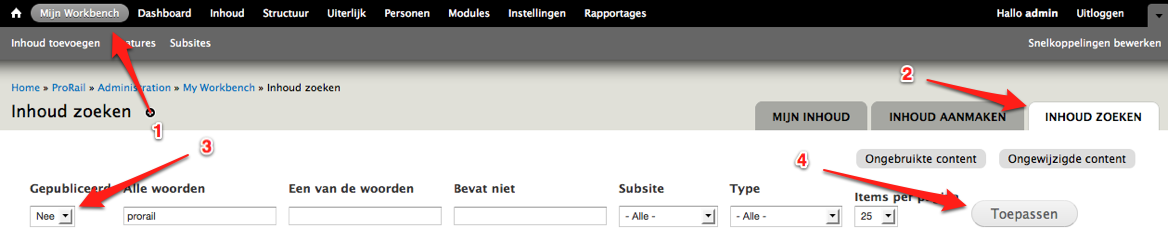
\includegraphics[width=\textwidth]{img/ongepubliceerdeinhoud.png}
\end{center}
De volgende filtering is mogelijk:
\begin{itemize}
\item Gepubliceerd \\
Hiermee kan worden gefilterd op alleen wel of niet gepubliceerde inhoud.
\item Alle woorden \\
Alle opgegeven woorden moeten voorkomen in de bodytekst. Woorden worden ook gevonden wanneer een deel van het woord is gegeven.
\item Een van de woorden \\
Minimaal \'{e}\'{e}n van de woorden moet voorkomen in de bodytekst.
\item Bevat niet \\
Deze tekst mag niet voorkomen in de bodytekst.
\item Subsite \\
Limiteer de resultaten tot een enkele subsite (doelgroep / project).
\item Type \\
Limiteer de resultaten tot een specifiek inhoudstype.
\end{itemize}
Daarnaast kan het aantal items per pagina worden opgegeven. Na het zoeken blijft de filtering staan en is het mogelijk om de opdracht te verfijnen door de filtering aan te passen. De sortering van de zoekresultaten kan worden aangepast door op de koppen van de tabel te klikken.

In het zoekresultaat verwijst de titel naar de pagina zelf. Daarnaast is er een bewerk-link beschikbaar. Na het bewerken van de node keert men terug naar de lijst met zoekresultaten. Bij het bezoeken van de pagina kan hiervoor de \emph{terug}-knop van de browser worden gebruikt.

\subsubsection{Ongebruikte content}
\pvelist{ \pve{2.9.6} }
Deze lijst bevat inhoud dat al enige tijd niet is bezocht. Het is te vinden onder \emph{Mijn Workbench} $\Rightarrow$ \emph{Inhoud zoeken} $\Rightarrow$ \emph{Ongebruikte content} of direct op \drupalpath{admin/workbench/all-content/unused}. Wanneer inhoud in deze lijst komt is afhankelijk van hoevaak deze tussentijds wordt bezocht. Wanneer deze nooit wordt bezocht dan komt deze na 3 maanden in de lijst. Het item zal nooit in de lijst komen wanneer deze grofweg dagelijks wordt bezocht..

\subsubsection{Ongewijzigde content}
\pvelist{ \pve{2.9.5} }
Deze pagina bevat een lijst met inhoud dat langer dan 6 maanden geleden voor het laatst is bewerkt. Het is te vinden onder \emph{Mijn Workbench} $\Rightarrow$ \emph{Inhoud zoeken} $\Rightarrow$ \emph{Ongewijzigde content} of direct op \drupalpath{admin/workbench/all-content/untouched}.

\subsection{Inhoud toevoegen}\label{inhoudtoevoegen}
\begin{enumerate}
\item Klik op de link "Inhoud" of ga direct naar \drupalpath{node/add}.
\item Klik op "Inhoud toevoegen", je zult nu een lijst te zien krijgen met alle content typen.
\item Klik vervolgens op het gewenste content type, je zult nu het scherm te zien krijgen waarin je de daadwerkelijke content kunt toevoegen.
\item Vul alle verplichte velden in (velden met een (*)).
\item Vul desgewenst de optionele velden in.
\item Om de pagina op te slaan klik je onderaan de pagina op de knop \emph{Opslaan}. Met deze actie wordt de pagina op de website direct bijgewerkt.
\end{enumerate}
%todo: screenshots

\subsection{Inhoud bewerken}
\pvelist{ \pve{2.2}, \pve{2.2.1}, \pve{2.2.2}, \pve{2.2.3}, \pve{2.2.4} }
Het bewerken van bestaande inhoud is voor een groot gedeelte gelijk aan het toevoegen van nieuwe inhoud. Tijdens het bewerken van de inhoud blijft de bestaande pagina zichtbaar voor bezoekers. De bezoekers zullen de wijzigingen pas zien nadat de pagina is opgeslagen en pas nadat de wijzigingen zijn goedgekeurd (indien workflow van toepassing is). Tevens zal de bezoeker (indien deze al op de pagina zit) handmatig de pagina moeten verversen voordat de nieuwe inhoud zichtbaar wordt.
\begin{enumerate}
\item Zoek de inhoud op via het dashboard\seeone{dashboard} of klik op de \emph{bewerken}-tab op de pagina zelf.
\item Er verschijnt eenzelfde scherm als bij het toevoegen van nieuwe inhoud. Alle velden zijn al ingevuld en kunnen worden aangepast.
\item Om de pagina op te slaan klik je onderaan de pagina op de knop \emph{Opslaan}. Met deze actie wordt de pagina op de website direct bijgewerkt.
\end{enumerate}


\subsection{Preview}
\pvelist{ \pve{2.3.2}, \pve{2.3.3}, \pve{2.3.4} }
Het is mogelijk om van nieuwe inhoud een preview te bekijken die de pagina laat zien alsof de laatste versie gepubliceerd is. Voordat deze preview is te zien moet de pagina wel worden opgeslagen, maar hoeft niet te worden gepubliceerd. De pagina kan dus worden opgeslagen als \emph{draft}\seeone{workflow}. Ga na het opslaan weer terug naar de bewerkpagina en klik onderaan op het tabblad "Voorbeeldweergave".

\subsubsection{Scheduler}
\pvelist{ \pve{2.3.1}, \pve{2.3.9}, \pve{2.9.2}, \pve{2.9.3} }
Het is mogelijk om vooraf een publicatiedatum in te stellen voor nieuwe en bestaande inhoud. Klik hiervoor bij het toevoegen of bewerken van inhoud op de tab \emph{Planneropties}. Hier kunnen twee data worden opgegeven; een datum voor publicatie en een datum voor depublicatie. Biede velden zijn optioneel en werken in principe onafhankelijk van elkaar. Bij het klikken op \'{e}\'{e}n van deze velden verschijnt er een kalender waarop de datum kan worden gekozen.
\begin{center}
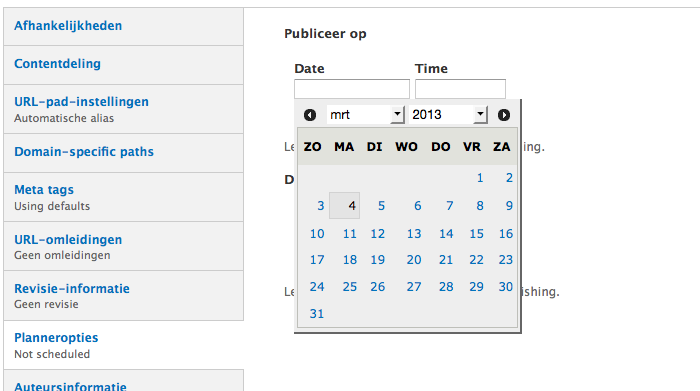
\includegraphics[width=\textwidth]{img/scheduler.png}
\end{center}
Niet gepubliceerde inhoud kan wel worden voorzien van tags, menu-items etc. Ook kunnen niet gepubliceerde items worden opgenomen in redactionele blokken\seeone{felix}. Zolang deze niet gepubliceerd is zal dit voor bezoekers niet zichtbaar zijn. Na publicatie (manueel of automatisch) wordt dit item zichtbaar.

Het (de)publiceren gebeurt in de cron (een achtergrond process dat om de 5 minuten draait) en kan daarom maximaal 5 minuten afwijken van de ingestelde tijd.


\subsection{Workflow en modereren/revisies}\label{workflow}
\pvelist{ \pve{2.2.5}, \pve{2.3.5}, \pve{2.3.6}, \pve{2.3.7}, \pve{2.3.10} }
In de website van ProRail wordt gebruik gemaakt van \emph{workflow}. Dat wil zeggen dat nieuwe inhoud en gewijzigde inhoud niet in alle gevallen direct op de site zal verschijnen, maar eerst goedgekeurd moet worden. Hierbij wordt onderscheid gemaakt tussen eindredacteuren en contentbeheerders. Contentbeheerders (ook wel "redacteur") kunnen enkel content binnen hun eigen subsite direct publiceren. Eindredacteuren hebben het recht om content binnen de gehele website te publiceren en aan te passen. Eindredacteuren kunnen content van contentbeheerders tevens publiceren op andere delen van de site.

De workflow is zowel van toepassing op nieuwe als bestaande inhoud. Bij reeds bestaande inhoud wordt een nieuwe \emph{revisie} aangemaakt. De nieuwe revisie kan bestaan naast de gepubliceerde pagina. Zo is het mogelijk dat een wijziging pas later - na goedkeuring - gepubliceerd wordt en dus zichtbaar voor bezoekers.

Bij het invoeren of bewerken van content is onderin het formulier een item "Publicatie-opties" te zien. Hierin staat een item "Moderatie status". Daarin zitten de volgende opties:
\begin{itemize}
\item Draft
\item Needs review
\item Published
\end{itemize}
Nieuwe inhoud of revisies worden als eerste aangemaakt als \emph{draft}. In deze staat is het een 'kladversie'. Bewerkingen hebben nog geen invloed op de website. Wanneer de content online mag dan kan de status op \emph{Needs review} worden gezet. In deze staat krijgen eindredacteuren dit item te zien in een lijst met goed te keuren inhoud. Tevens wordt een mail gestuurd naar alle eindredacteuren. Het item kan daarna op \emph{Published} worden gezet. De inhoud wordt dan zichtbaar op de website voor alle bezoekers. Afhankelijk van de rechten is het mogelijk om in dit proces stappen over te slaan.

\subsubsection{Revisies inzien en terugzetten}\label{modererentab}

De revisies van inhoud zijn later (ook na publicatie) terug te vinden onder het tabblad "Modereren". Op deze pagina is een lijst te zien waarin tevens de datum en workflow status te zien is. Met de link "weergeven" kan de revisie worden bekeken. Met de link "terugzetten" kan de revisie worden teruggezet. In het laatste geval publiceren we een oudere revisie, waarmee we alle latere wijzigingen ongedaan maken. Een revisie kan ook nieuwer zijn dan de versie die is gepubliceerd. In dit geval is er een "publiceren" link aanwezig. Hiermee kan deze versie worden goedgekeurd en gepubliceerd.

Onder de link "Vergelijk revisies" (2e niveau tabblad) zit een pagina waarmee makkeljik te verschillen tussen revisies zichtbaar gemaakt kunnen worden. Hierbij moeten twee revisies gekozen worden. Kies eerst de nieuwste revisie en daarna de oudere revisie (verder onderaan in de lijst). Klik daarna op de knop \emph{Vergelijken}. Hierna worden de tekstuele wijzigingen getoond. Dit heeft betrekking op de hoofdtekst van dit item.
\begin{center}
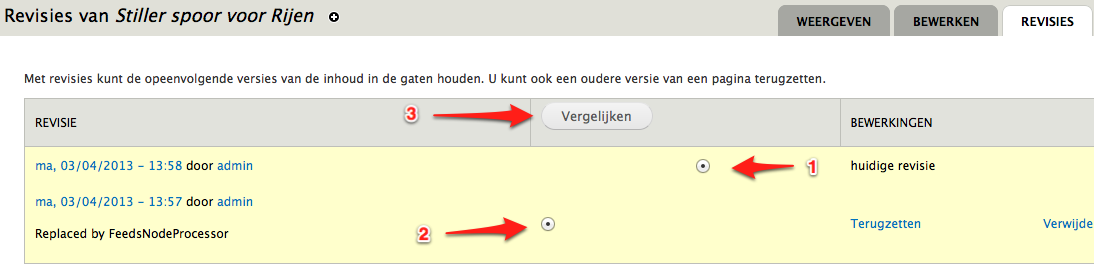
\includegraphics[width=\textwidth]{img/revisies3.png}
\end{center}

\subsubsection{Inhoud goedkeuren}

In het dashboard is voor eindredacteuren een lijst beschikbaar met inhoud dat goedgekeurd dient te worden. Dit is inhoud met de status \emph{Needs review}. Klik hiervoor linksboven op "Mijn Workbench" en dan op "Wacht op goedkeuring" (2e niveau tabblad). In deze lijst kan doorgeklikt worden naar de pagina's die goedgekeurd dienen te worden. Nadat de wijzigingen zijn bekeken kunnen deze worden goedgekeurd onder het tabblad "Modereren"\see{modererentab}.


\subsection{Contenttypes}

\subsubsection{Wiki}

Wiki

\subsubsection{Poll}
\pvelist{ \pve{4.26} }
Ga naar Inhoud $\Rightarrow$ Inhoud toevoegen $\Rightarrow$ Enqu\^{e}te, of direct naar drupalpath{node/add/advpoll}. De volgende velden zijn beschikbaar.
\begin{enumerate}
\item Vraag, de vraag en tevens titel van de poll.
\item Beschrijving, een eventuele omschrijving bij de vraag.
\item Poll choice, de antwoorden waarop een gebruiker kan stemmen. Via de knop Item toevoegen kan je extra vragen toevoegen.
\item Poll availability, kies hier tussen welke data de poll open moet zijn. Buiten deze periode is de poll nog wel zichtbaar maar kan er niet gestemd worden.
\item Close poll, kies hier of de poll open en gesloten moet zijn. Je kan hiermee de poll sluiten ook wanneer hij nog binnen het termijn valt.
\end{enumerate}

Via Felix kan een poll worden geplaatst op de website.


\subsubsection{Carousel}
\pvelist{ \pve{4.14} }
\begin{enumerate}
\item Klik op de link \emph{Inhoud toevoegen} of ga direct naar \
\item Vul de titel in van de slide
\item Klik op de \emph{Select media} button om een afbeelding te kiezen
\item Klik op \emph{Library} om een afbeelding te gebruiken die eerder is toegevoegd,  of voeg een nieuwe afbeelding toe via \emph{Upload a new file}
\item Vul een url in bij het \emph{Link} veld
\item Om de pagina op te slaan klik je onderaan de pagina op de knop \emph{Opslaan}
\item Om de slide aan een carousel toe te voegen wordt uitgelegd in \seeone{nodequeues}
\end{enumerate}
%todo: screenshots

\subsubsection{Systeempagina}
\pvelist{ \pve{2.6.4} }
Systeempagina's zijn gelijk aan een standaard pagina\seeone{pagenode} met het verschil dat een systeempagina niet wordt opgenomen in de zoekresultaten. Dit wordt bijvoorbeeld gebruikt voor de foutpagina's, maar kan door redacteuren ook voor andere pagina's worden gebruikt waarvan niet wenselijk is dat deze in de zoekresultaten voorkomen.

\subsubsection{Cookiebalk}
Via \drupalpath{admin/config/user-interface/cookie-consent} kunnen de instellingen voor de cookiebalk worden aangepast. Hier kan bijvoorbeeld de link voor meer informatie worden aangepast. Ook kunnen domeinen uitgesloten worden van deze functionaliteit (dient alleen gebruikt te worden voor domeinen die niet publiekelijk bereikbaar zijn).

\subsubsection{Hoofdnavigatie}
%todo: screenshots

\subsubsection{Toevoegen FAQ}

\begin{enumerate}
\item Ga naar Inhoud $\Rightarrow$ Inhoud toevoegen $\Rightarrow$ FAQ of direct naar \drupalpath{/node/add/faq}.
\item De volgende velden kunnen ingevoerd worden; vraag en body.
\end{enumerate}

\subsubsection{Koppelen van een FAQ aan content}

\begin{enumerate}
\item Bewerk of maak een nieuwe node aan.
\item Bij het onderdeel Koppel FAQ kan je middels een autocomplete veld vragen zoeken en koppelen aan het item.
\item Sla daarna de node op.
\end{enumerate}